%//////////////////////////////////
%/// P R E A M B L E

\documentclass[a4paper, 12pt]{article}

\usepackage[utf8]{inputenc}
\usepackage[singlespacing]{setspace}
\usepackage{amsmath}
\usepackage{mathtools}
\usepackage{caption}
\usepackage{float}
\usepackage{booktabs}
\usepackage{graphicx}
\usepackage{multicol}
\usepackage{gensymb}
\usepackage{breqn}
\usepackage{indentfirst}
\usepackage{siunitx}
\usepackage{tabularx, booktabs}
\newcolumntype{Y}{>{\centering\arraybackslash}X}

\usepackage{pdfpages}

\usepackage{multicol}
\usepackage{supertabular}

\usepackage{svg}

\widowpenalty = 4500
\clubpenalty  = 4500

\setlength{\jot}{10pt} %indents


\newcommand*\dif{\mathop{}\!\mathrm{d}}
%\newcommand{\euler}{\mathrm{e}}
%\newcommand{\ramuno}{\mathrm{j}}

%%========================================
%% circuitikz properties
\usepackage[european, straightvoltages]{circuitikz}
%\ctikzvalof{voltage/distance from node = .2}
%\ctikzset{voltage/distance from node  =.5}% in \pgf@circ@Rlen units
%\ctikzset{voltage/distance from line  =.25}% pos. between 0 and 1
%\ctikzset{voltage/bump b/.initial     =1.5}%

\ctikzset{current/distance            = .618}


%%========================================

%%
%% Path settings
%%
\graphicspath{ {./graphics/} }


%//////////////////////////////////
%/// D O C U M E N T
\begin{document}

%%%%%%%%%%%%%%%%%%%%%%%%%%%%%%%%%%%%%
  %\includepdf{Deckblatt.pdf}
  
\includepdf{./titlepage/titlepage.pdf}
%%%%%%%%%%%%%%%%%%%%%%%%%%%%%%%%%%%%%

\section{Vorbereitungsaufgaben}

  %1.1
  \subsection{}
    \begin{center}
      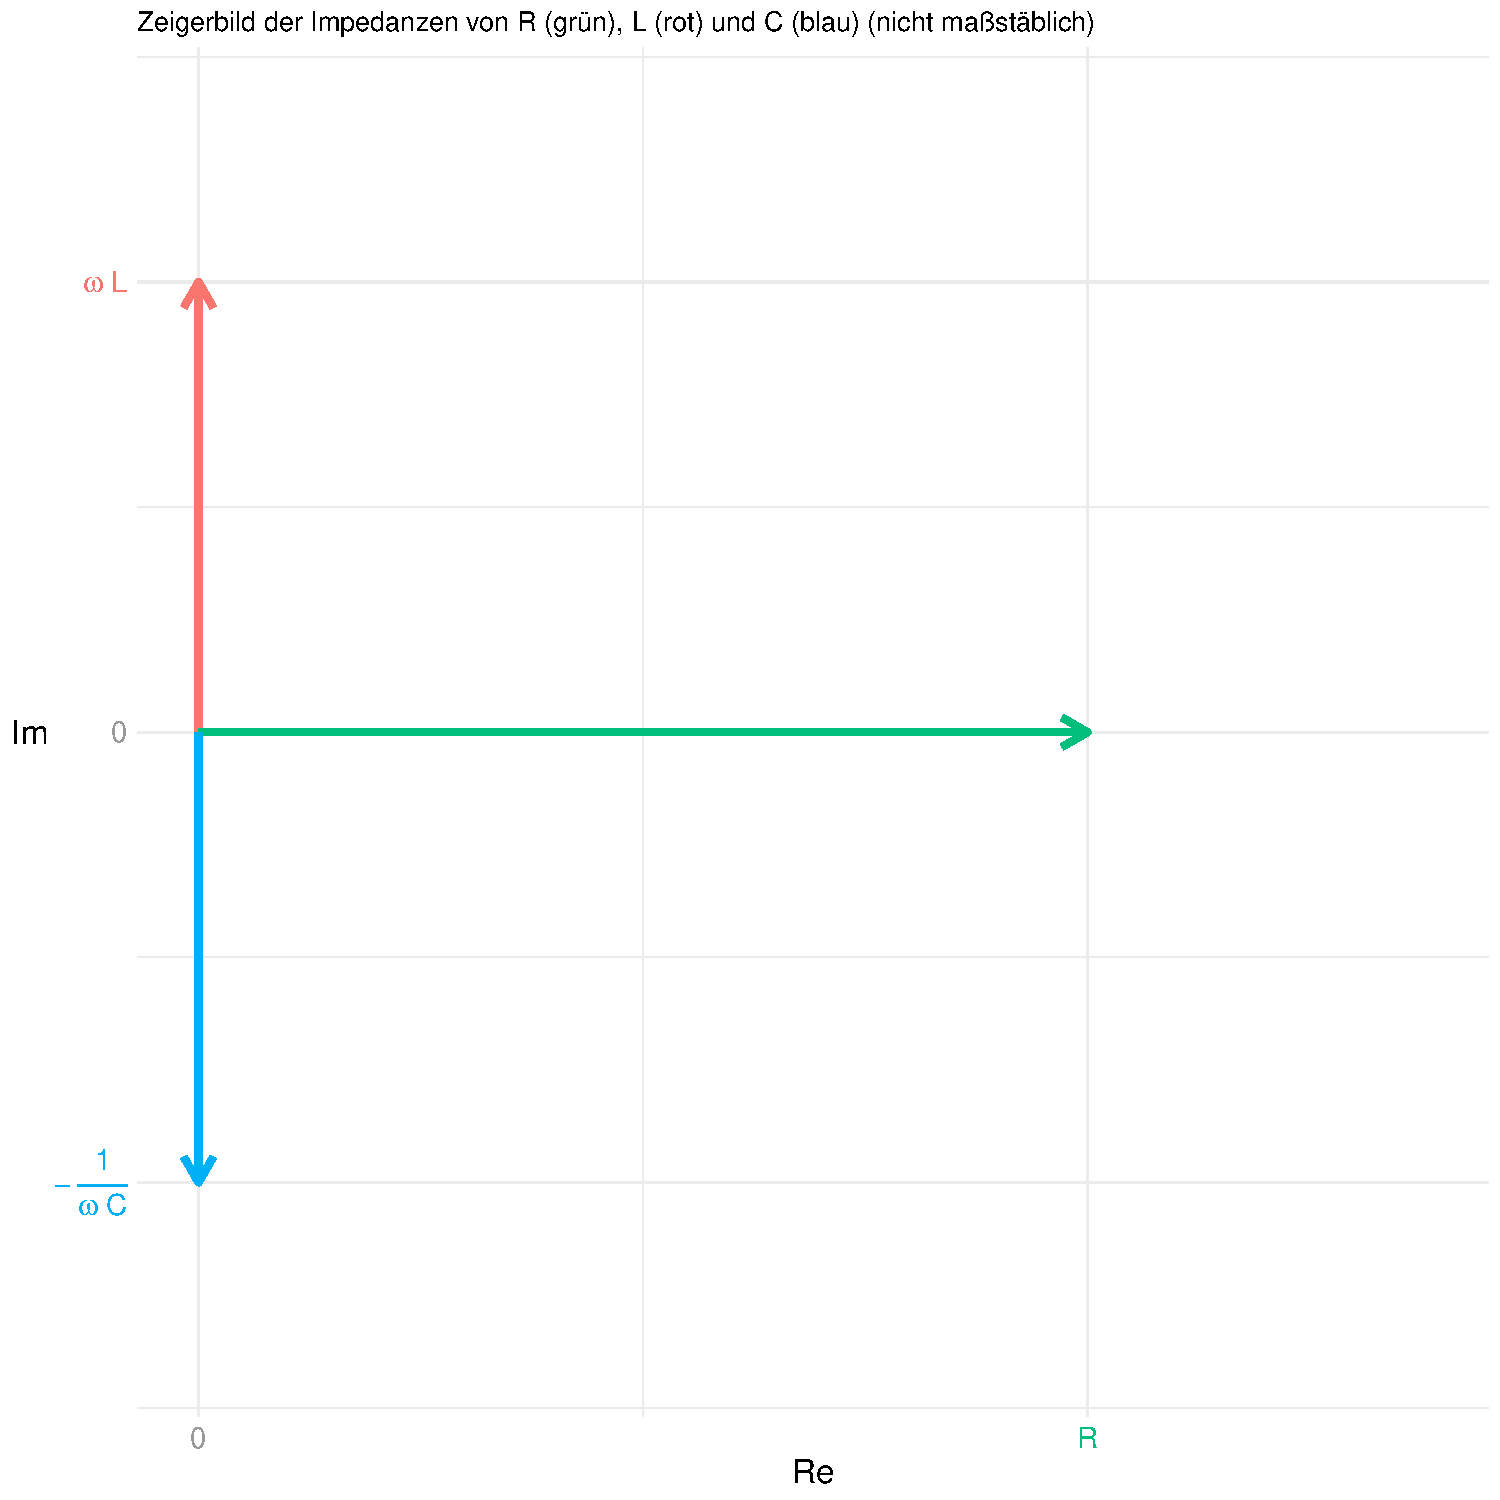
\includegraphics[scale=0.5]{./R/2_1/RLC_Zeiger_Impedanz.pdf}\\
      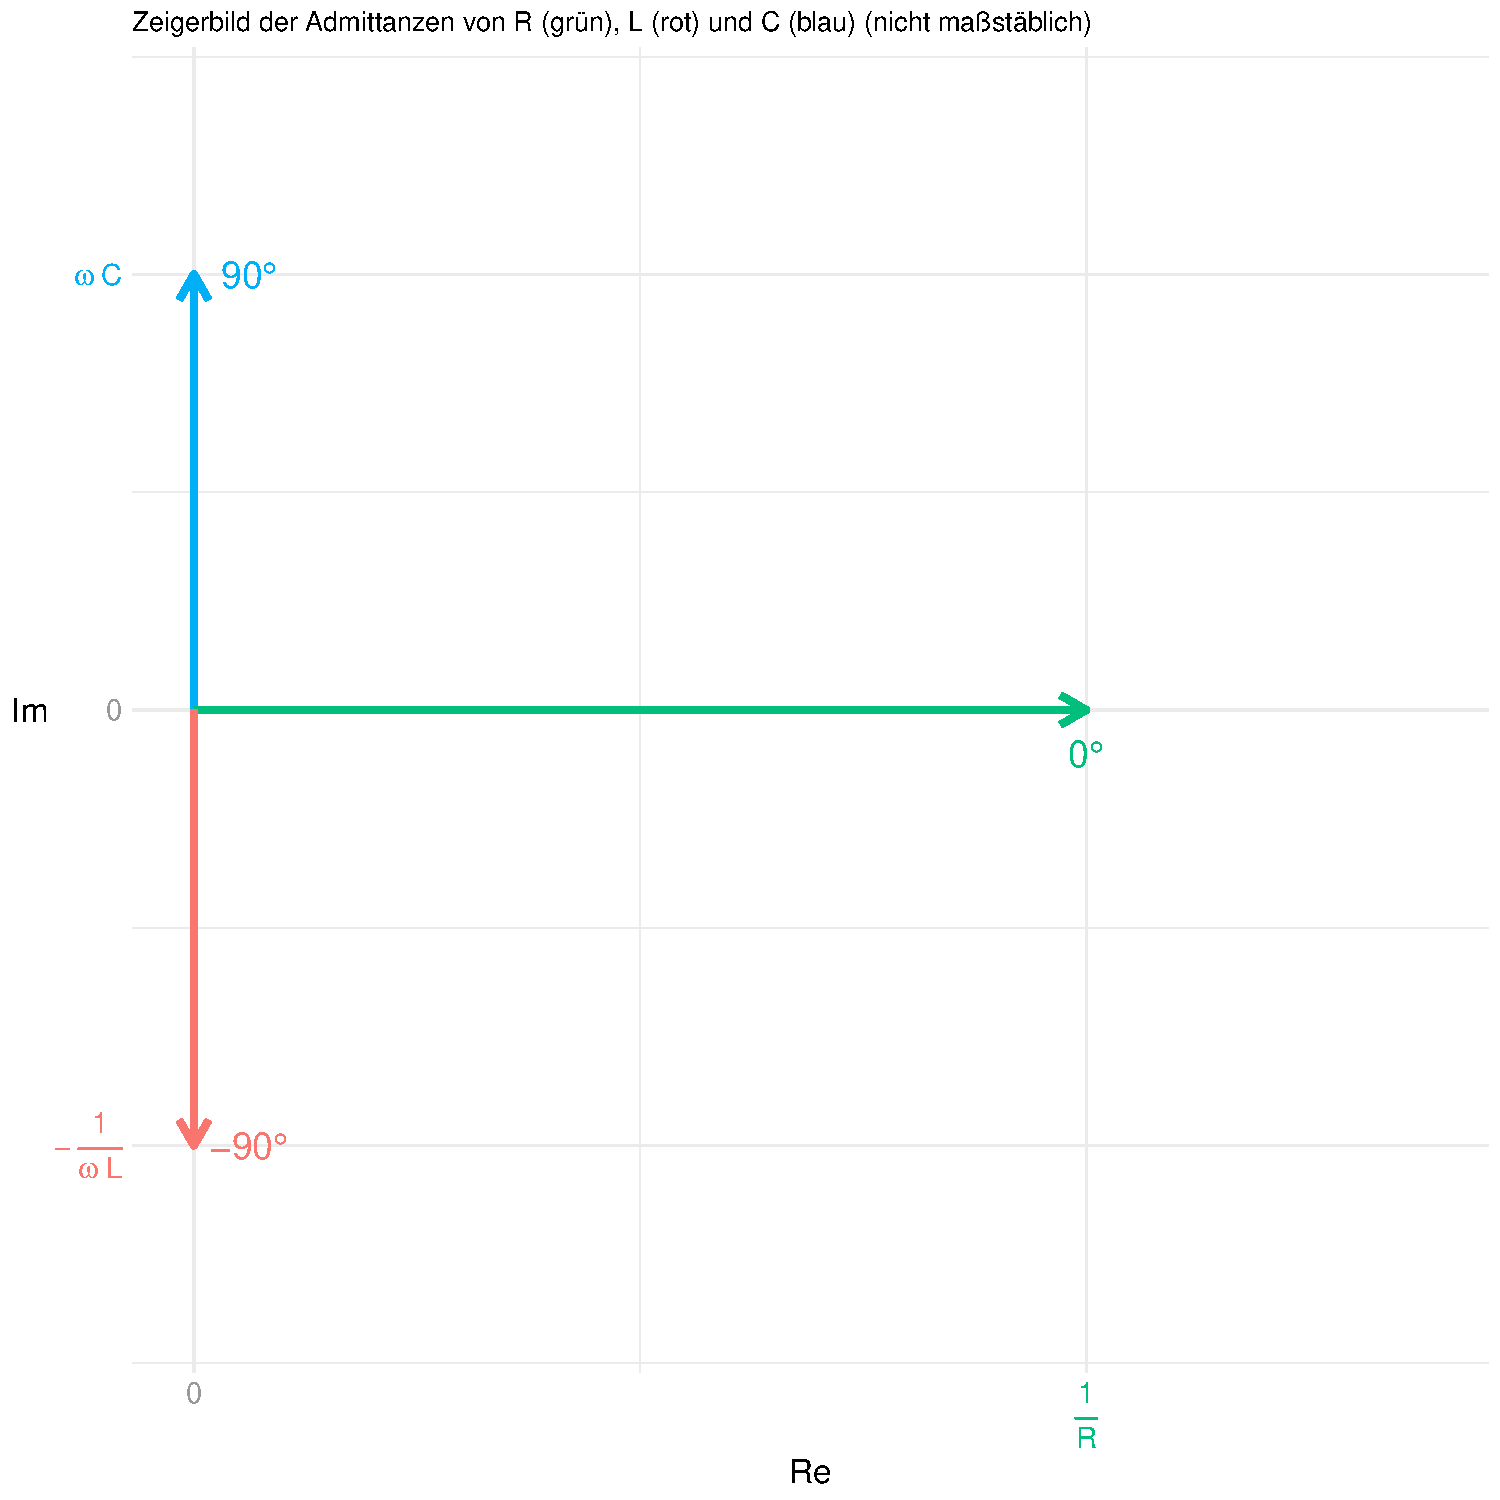
\includegraphics[scale=0.5]{./R/2_1/RLC_Zeiger_Admittanz.pdf}
    \end{center}

  %1.2
  \subsection{}

    \begin{center}
      \begin{circuitikz}

        \draw (0,0) to[R, l=$R$, o-] (2,0);
        \draw (2,0) to[L, l=$L$, i=$\underline{I}$] (6,0);
        \draw (6,0) to[C, l=$C$, -o] (8,0);

      \end{circuitikz}
    \end{center}

    \begin{gather*}
      \underline{I} = \frac{\underline{U}}{\underline{Z}},\,\ \underline{U} = \hat{U} \cdot e^{j(\omega t + \phi_u)}\\
      \underline{Z} = R + j \omega L + \frac{1}{j \omega C}\\
      \underline{I} = \frac{\hat{U} \cdot e^{j(\omega t + \phi_u)}}{R+j (\omega L - \frac{1}{ \omega C})}
      \intertext{Betrag:}
      \mid \underline{I} \mid = \hat{I} = \frac{\hat{U}}{\sqrt{R^2 + (\omega L - \frac{1}{\omega C} )^2}}
      \intertext{Phase:}
      \phi_i = \phi_u - \arctan{\left(\frac{\omega L - \frac{1}{\omega C} }{R} \right)}
      \intertext{Gesamt:}
      i(t) = \frac{\hat{U}}{\sqrt{R^2 + (\omega L - \frac{1}{\omega C} )^2}} \cdot \cos{\left( \omega t +  \phi_u - \arctan{\left(\frac{\omega L - \frac{1}{\omega C} }{R} \right)}\right)}
    \end{gather*}

  %1.3
  \subsection{}
    \begin{center}
      \begin{circuitikz}

        \draw (0,0) to[R, l=$R_{sL}$,v=$U_{R_{\text{eff}}}$, o-] (2,0)
        to[L, l=$L$, -o, v=$U_{L_{\text{eff}}}$, i=$i_{\text{eff}}$] (4,0);

      \end{circuitikz}
      \vspace{0.021276873\paperheight}
    $$I = 1.5 \,\ \si{\milli\ampere}, \,\ R_{sL}=200 \si{\ohm},\,\ L = 60 \,\ \si{\milli\henry}$$ \end{center}

    \begin{gather*}
      \underline{U}_{\text{ges}}=\underline{I}\cdot(R_{sL}+j \omega L)\\
      \hat{U}_{\text{ges}} = \hat{I} \cdot \sqrt{R_{sL}^2 + \omega^2 L^2}\\
      \hat{U}_{\text{ges}_{\text{eff}}}
      = I_{\text{eff}}\cdot \sqrt{R_{sL}^2 + \omega^2 L^2}
      = 1.5 \si{\milli\ampere} \cdot \sqrt{(200 \si{\ohm})^2 + 4 \pi^2 f^2 \cdot (60 \si{\milli\henry})^2 }
    \end{gather*}

    \begin{gather*}
      U_{R_{\text{eff}}} = I_{\text{eff}} \cdot R = 1.5 \si{\milli\ampere} \cdot 200 \si{\ohm} = 0.3 \,\ \si{\volt}
    \end{gather*}

    \begin{gather*}
      U_{L_{\text{eff}}} = I_{\text{eff}} \cdot \omega L = 1.5 \si{\milli\ampere} \cdot 2 \pi f \cdot 60 \si{\milli\henry}
    \end{gather*}

    \begin{center}
      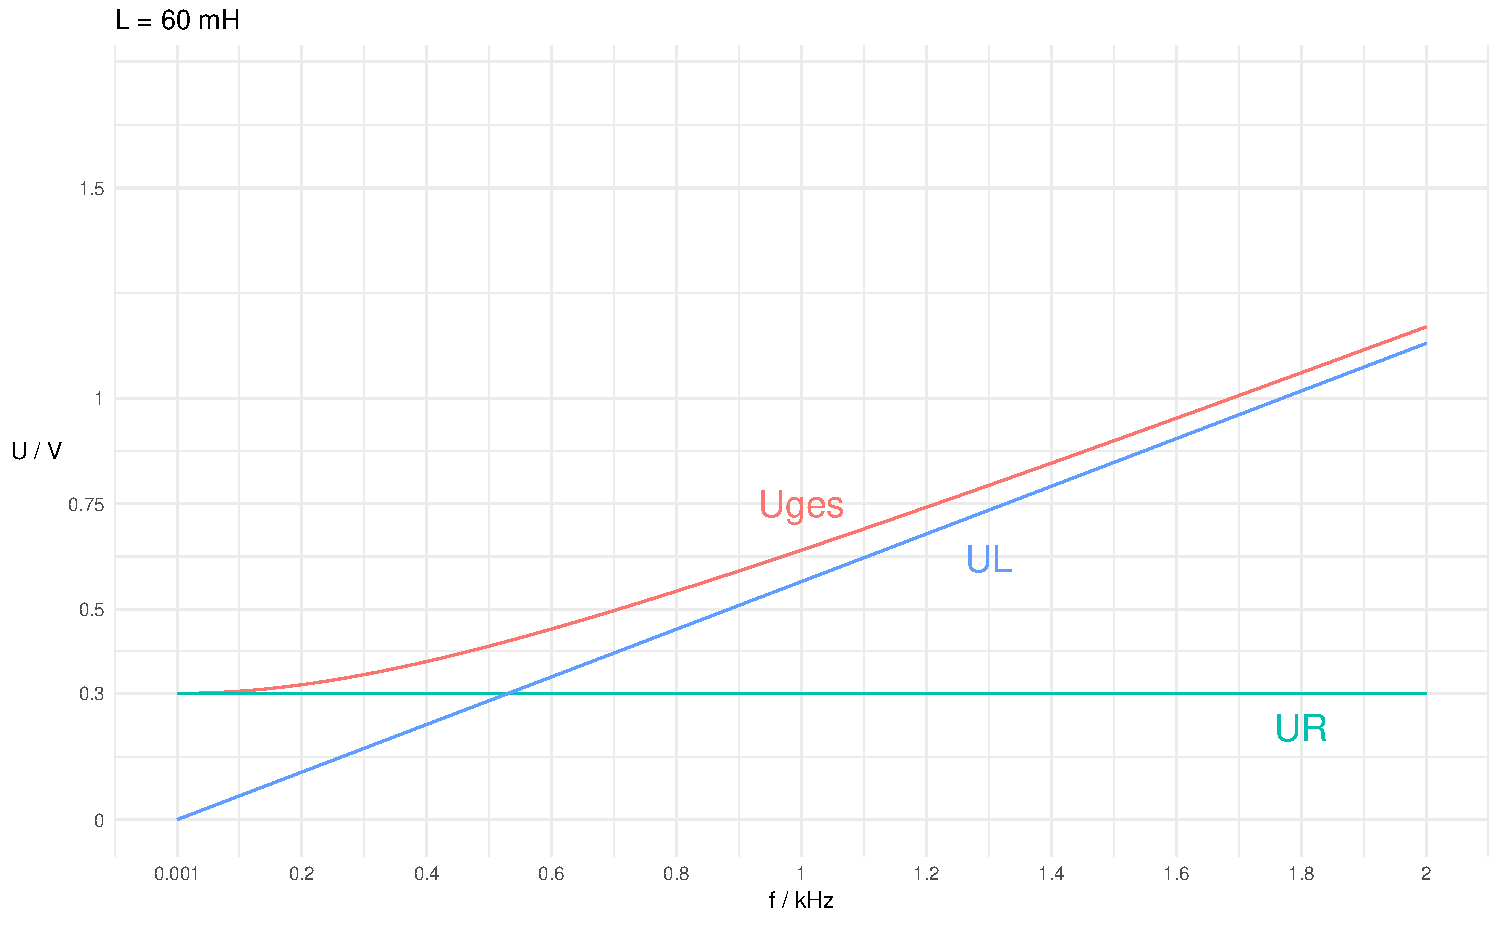
\includegraphics[scale=0.5]{./R/2_3/2_3.pdf}
    \end{center}

  %1.4
  \subsection{}
    \begin{center}
      \begin{circuitikz}

        \draw (0,0) to[R, l=$R$,v=$U_{R_{\text{eff}}}$, o-] (2,0)
        to[C, l=$C$, -o, v=$U_{C_{\text{eff}}}$, i=$i_{\text{eff}}$] (4,0);

      \end{circuitikz}
      \vspace{0.021276873\paperheight}
      $$I = 1.5 \,\ \si{\milli\ampere}, \,\ R=200 \si{\ohm},\,\ C_1 = 0.5 \,\ \si{\micro\farad}, \,\ C_2 = 1 \,\ \si{\micro\farad}$$\end{center}

    \begin{gather*}
      \underline{U}_{\text{ges}}=\underline{I}\cdot(R-j\frac{1}{\omega C})\\
      \hat{U}_{\text{ges}} = \hat{I} \cdot \sqrt{R^2 + \frac{1}{\omega^2 C^2} }\\
      \hat{U}_{\text{ges}_{\text{eff}}}=I_{\text{eff}}\cdot\sqrt{R^2 + \frac{1}{\omega^2 C^2} } = 1.5 \si{\milli\ampere} \cdot \sqrt{(200 \si{\ohm})^2 + \frac{1}{4 \pi^2 f^2 C^2} }
    \end{gather*}

    \begin{gather*}
      U_{R_{\text{eff}}} = I_{\text{eff}} \cdot R = 1.5 \si{\milli\ampere} \cdot 200 \si{\ohm} = 0.3 \,\ \si{\volt}
    \end{gather*}

    \begin{gather*}
        U_{C_{\text{eff}}} = I_{\text{eff}} \cdot \frac{1}{\omega C}\\
        U_{C_{{\text{eff}}_1}} = I_{\text{eff}} \cdot \frac{1}{\omega C_1} = 1.5 \si{\milli\ampere} \cdot \frac{1}{2 \pi f \cdot 0.5 \si{\micro\farad}}\\
        U_{C_{{\text{eff}}_2}} = I_{\text{eff}} \cdot \frac{1}{\omega C_2} = 1.5 \si{\milli\ampere} \cdot \frac{1}{2 \pi f \cdot 1 \si{\micro\farad}}
    \end{gather*}

    \begin{center}
      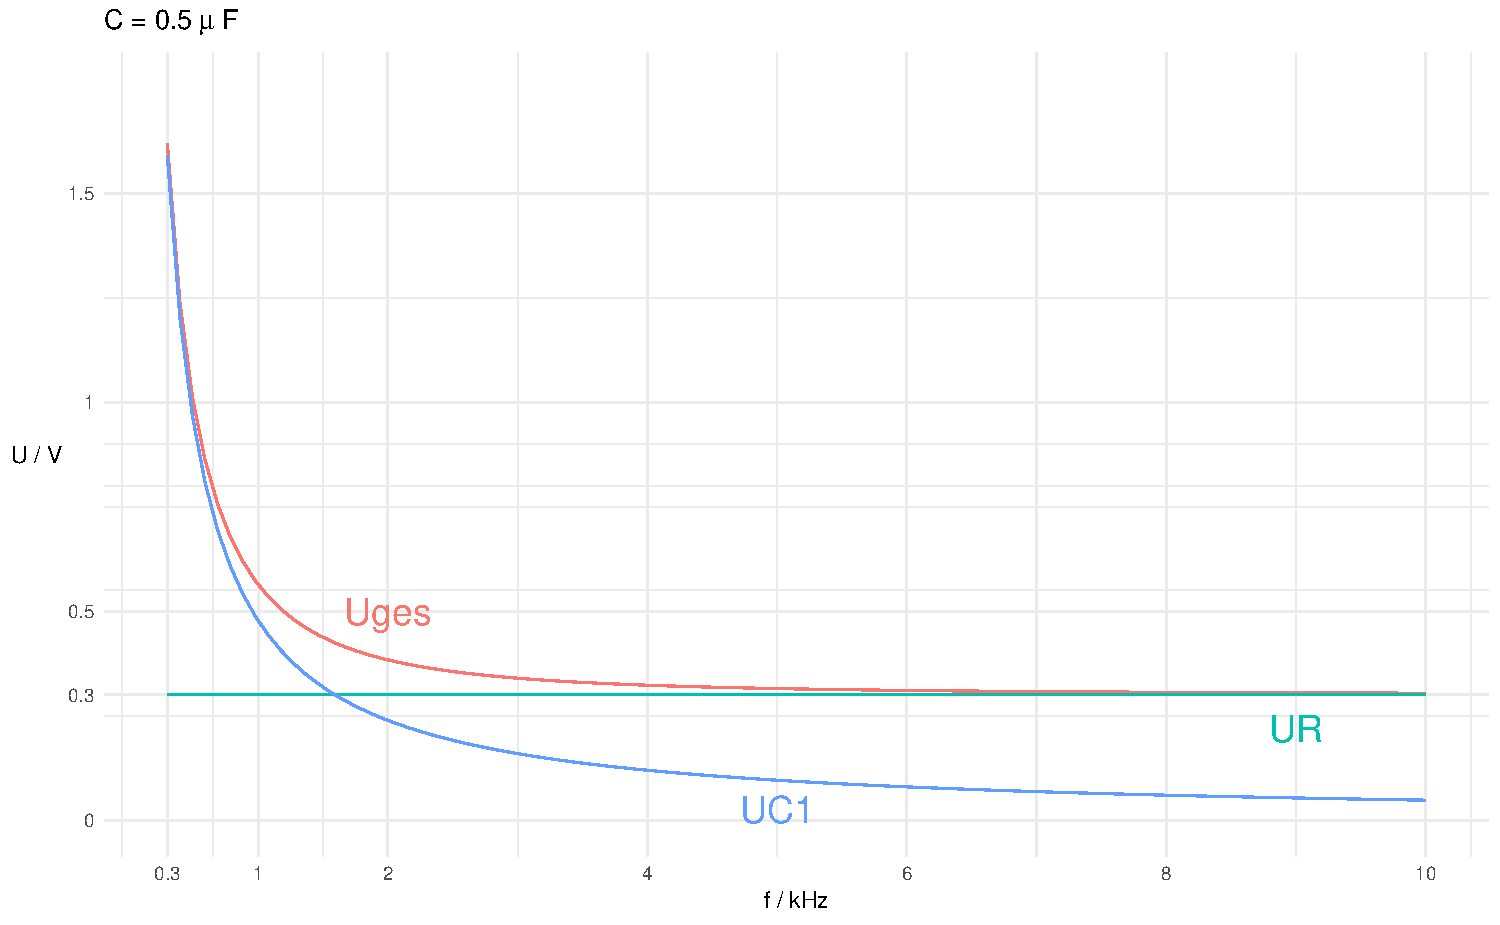
\includegraphics[scale=0.5]{./R/2_4/2_4_1.pdf}\\
      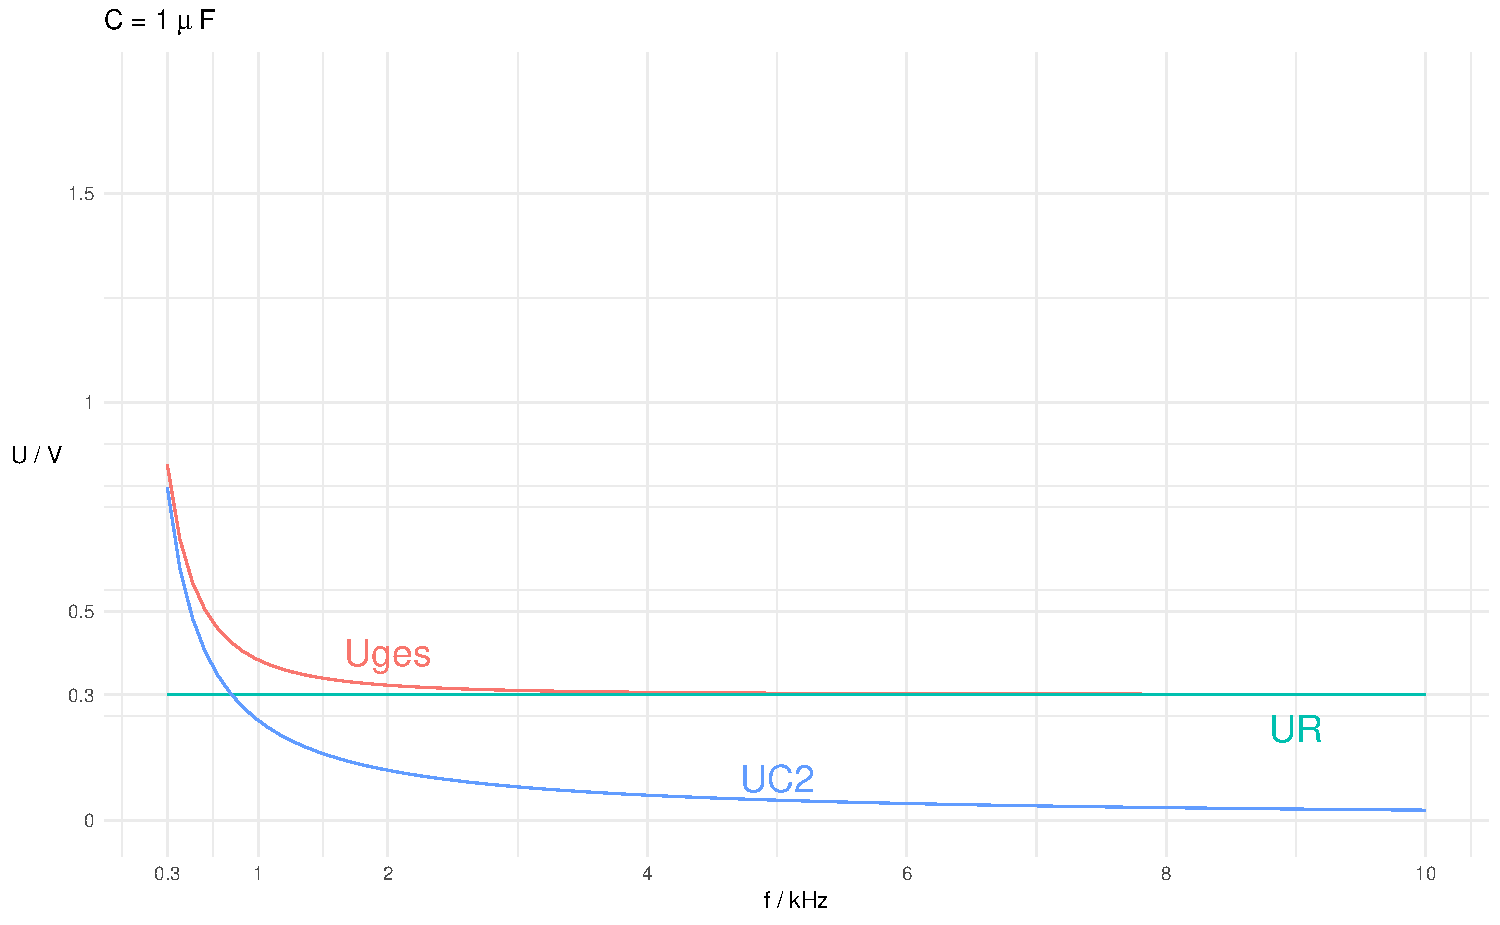
\includegraphics[scale=0.5]{./R/2_4/2_4_2.pdf}
    \end{center}

  %1.5
  \subsection{}
    \subsubsection*{a) Spule}

      %%%%%%%%%%%%%%%%%%%%%%%%%%%%%%%%%%%%%%%%%%%%%
        \begin{center}
          \begin{circuitikz}

            \draw (0,0) to[R, l=$R_{sL}$, o-] (2,0)
            to[L, l=$L_s$, -o] (4,0);

          \end{circuitikz}
        \end{center}
        \vspace{0.021276873\paperheight}

        \begin{center}
          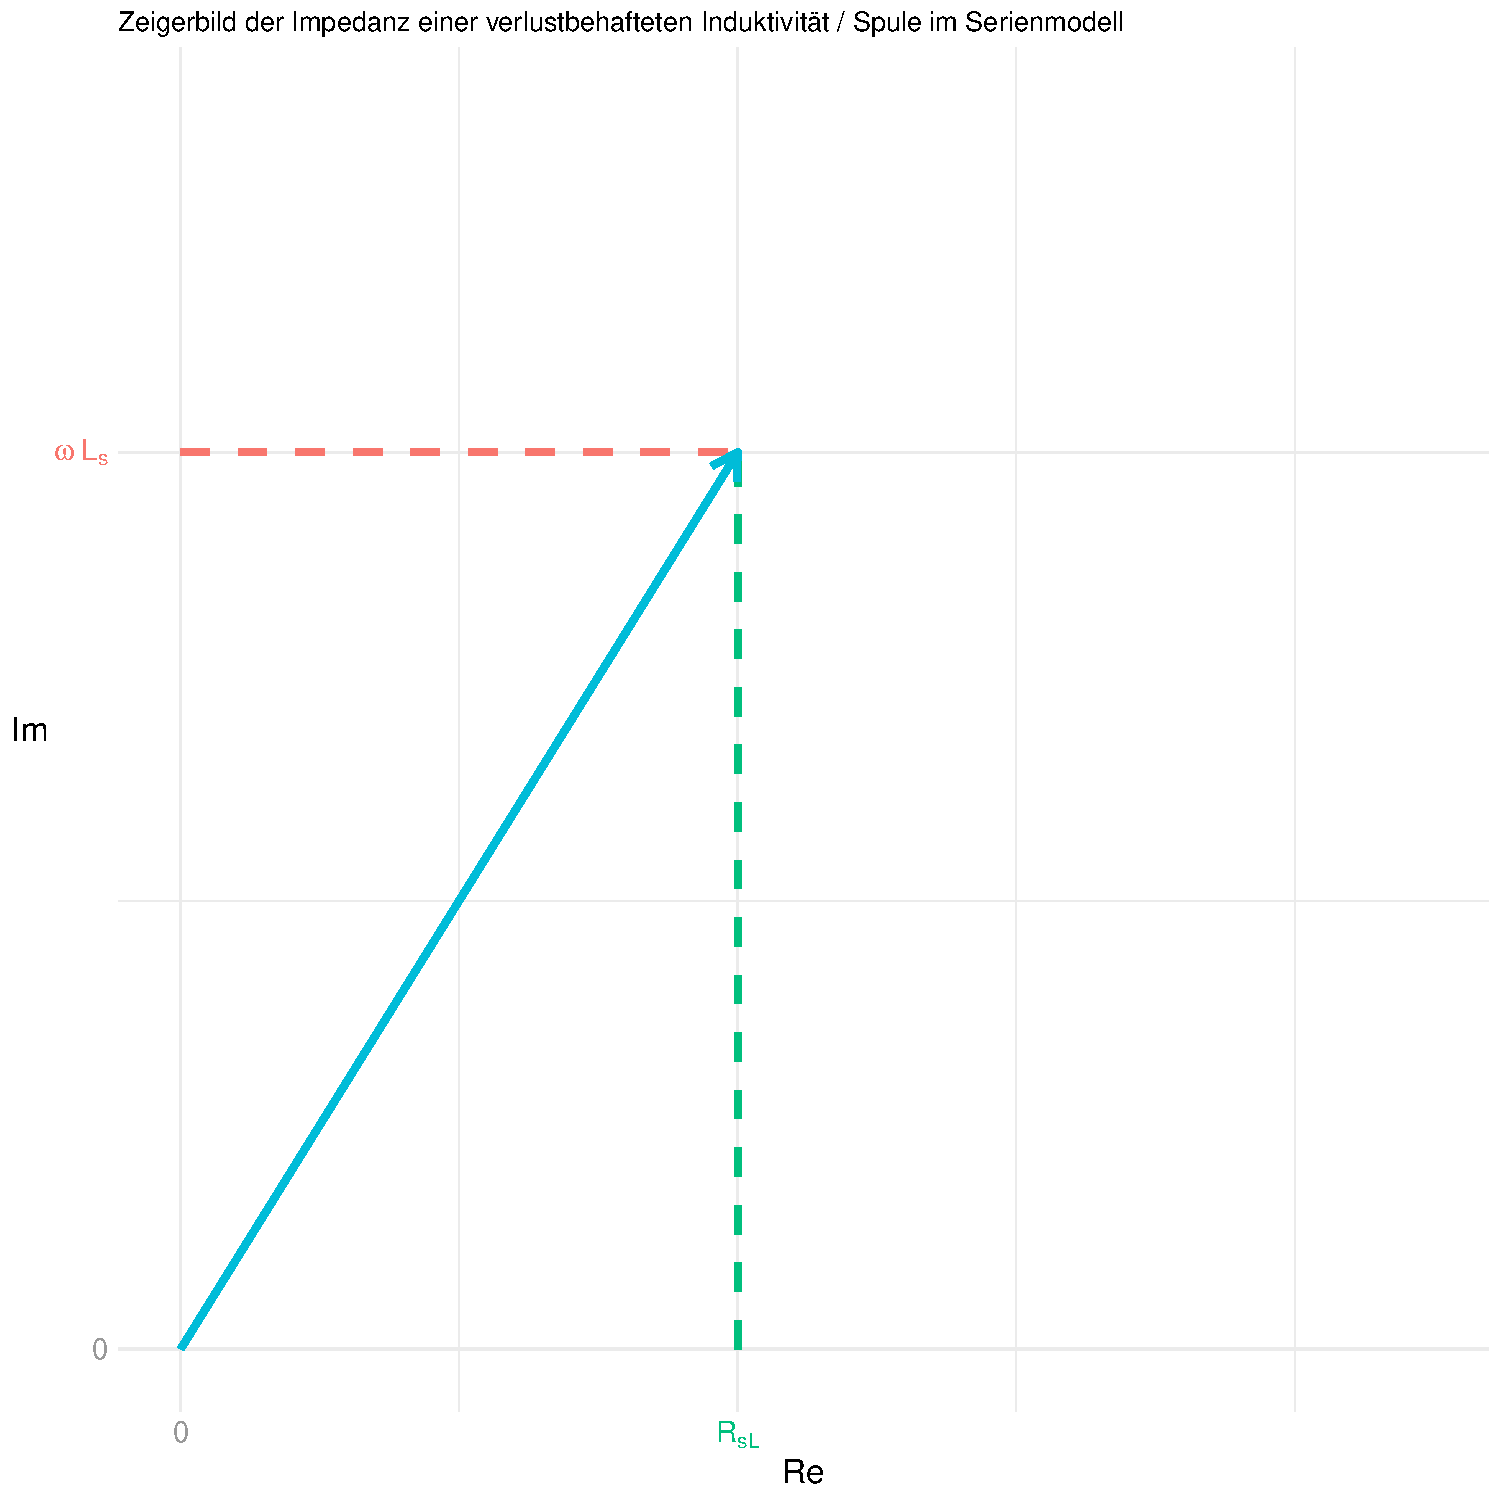
\includegraphics[scale=0.5]{./R/2_5/RL_Zeiger.pdf}
        \end{center}

        Der Winkel $\delta$, den die Impedanz $\underline{Z}$ mit der imaginären Achse bildet, wird Verlustwinkel genannt. Der Verlustfaktor $d$ ergibt sich dann aus:
        $$d = \tan{\delta} = \frac{R_{sL}}{L_s} $$

        \noindent Die Güte $Q$ ist definiert als der Kehrwert des Verlustfaktors, also:
        $$Q_{Ls} = \frac{1}{d} = \frac{\omega L_s}{R_{sL}} $$


      %%%%%%%%%%%%%%%%%%%%%%%%%%%%%%%%%%%%%%%%%%%%%
        \vspace{0.021276873\paperheight}
        \begin{center}
          \begin{circuitikz}

            \draw (0,0) -- (1,0);
            \draw (1,-1) -- (1,1);
            \draw (1,1) to[R, l=$R_{pL}$] (4,1);
            \draw (1,-1) to[L, l=$L_p$] (4,-1);
            \draw (4,-1) -- (4,1);
            \draw (4,0) -- (5,0);


          \end{circuitikz}
        \end{center}
        \vspace{0.021276873\paperheight}

        \begin{center}
          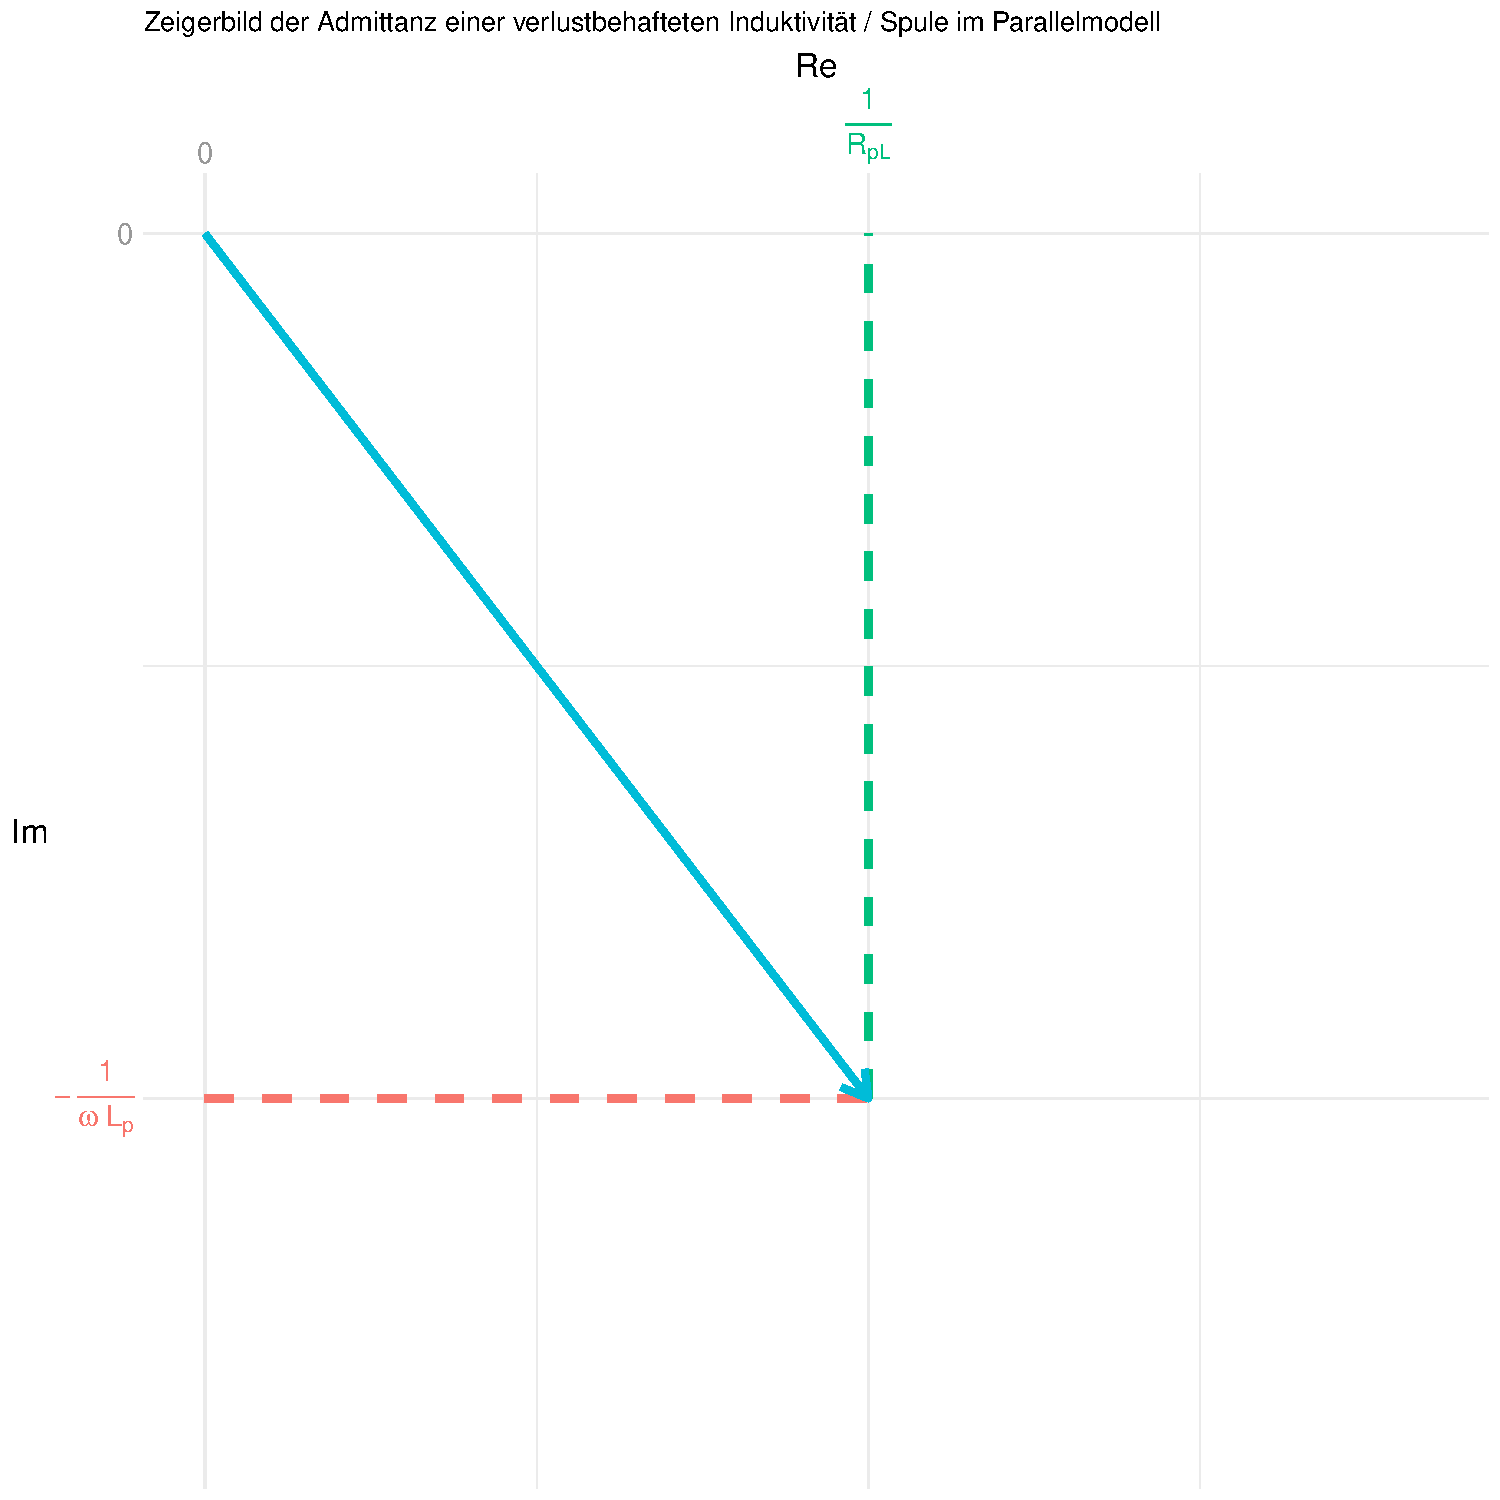
\includegraphics[scale=0.5]{./R/2_5/RL_Zeiger_parallel.pdf}
        \end{center}

        Analog ist der Verlustwinkel $\delta$ der Winkel der Admittanz mit der imaginären Achse:
        $$ d = \tan{\delta} = \frac{ \frac{1}{R_{pL}} }{ \mid - \frac{1}{\omega L_p} \mid} = \frac{\omega L_p}{R_{pL}} $$

        \noindent Demnach ist auch die Güte der Kehrwert des Verlustfaktors:
        $$Q_{Lp} = \frac{1}{d} = \frac{R_{pL}}{\omega L_p} $$

        \noindent Für die gleich Frequenz gilt damit:
        $$Q_{L_s} = Q_{L_p} = Q_L$$
      %%%%%%%%%%%%%%%%%%%%%%%%%%%%%%%%%%%%%%%%%%%%%
    \pagebreak{}
    \subsubsection*{b) Kondensator}

      \begin{center}
        \begin{circuitikz}

          \draw (0,0) to[R, l=$R_{sC}$, o-] (2,0)
          to[C, l=$C_s$, -o] (4,0);

        \end{circuitikz}
      \end{center}
      \vspace{0.021276873\paperheight}

      \begin{center}
        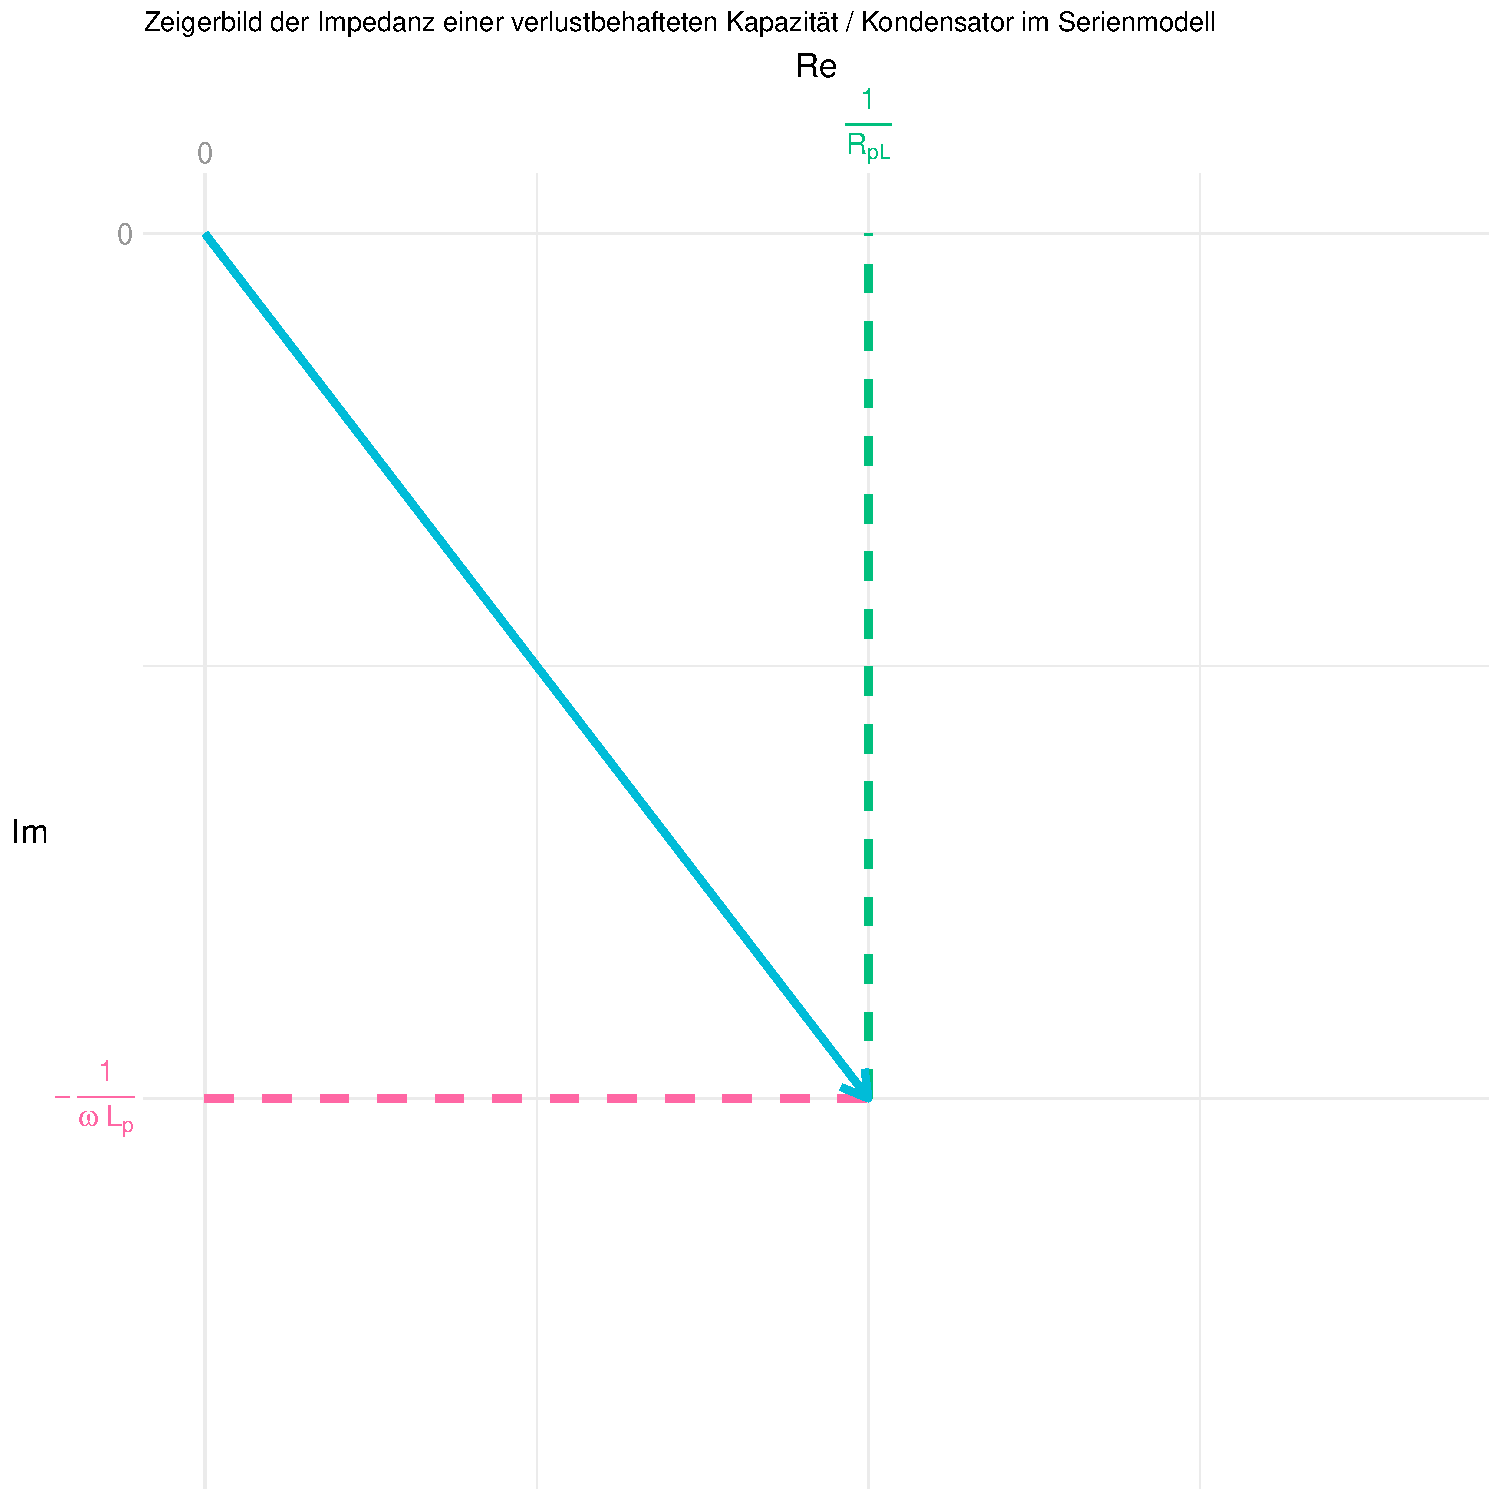
\includegraphics[scale=0.5]{./R/2_5/RC_Zeiger.pdf}
      \end{center}

      Der Winkel $\delta$, den die Impedanz $\underline{Z}$ mit der imaginären Achse bildet, wird Verlustwinkel genannt. Der Verlustfaktor $d$ ergibt sich dann aus:
      $$d = \tan{\delta} = \frac{R_{sC}}{\mid -\frac{1}{\omega C_s }\mid} = R_{sC} \cdot \omega C_s$$

      \noindent Die Güte $Q$ ist definiert als der Kehrwert des Verlustfaktors, also:
      $$Q_{Cs} = \frac{1}{d} = \frac{1}{\omega R_{sC} C_s} $$

      %%%%%%%%%%%%%%%%%%%%%%%%%%%%%%%%%%%%%%%%%%%%%
      \vspace{0.021276873\paperheight}
      \begin{center}
        \begin{circuitikz}

          \draw (0,0) -- (1,0);
          \draw (1,-1) -- (1,1);
          \draw (1,1) to[R, l=$R_{pC}$] (4,1);
          \draw (1,-1) to[C, l=$C_p$] (4,-1);
          \draw (4,-1) -- (4,1);
          \draw (4,0) -- (5,0);

        \end{circuitikz}
      \end{center}
      \vspace{0.021276873\paperheight}

      \begin{center}
        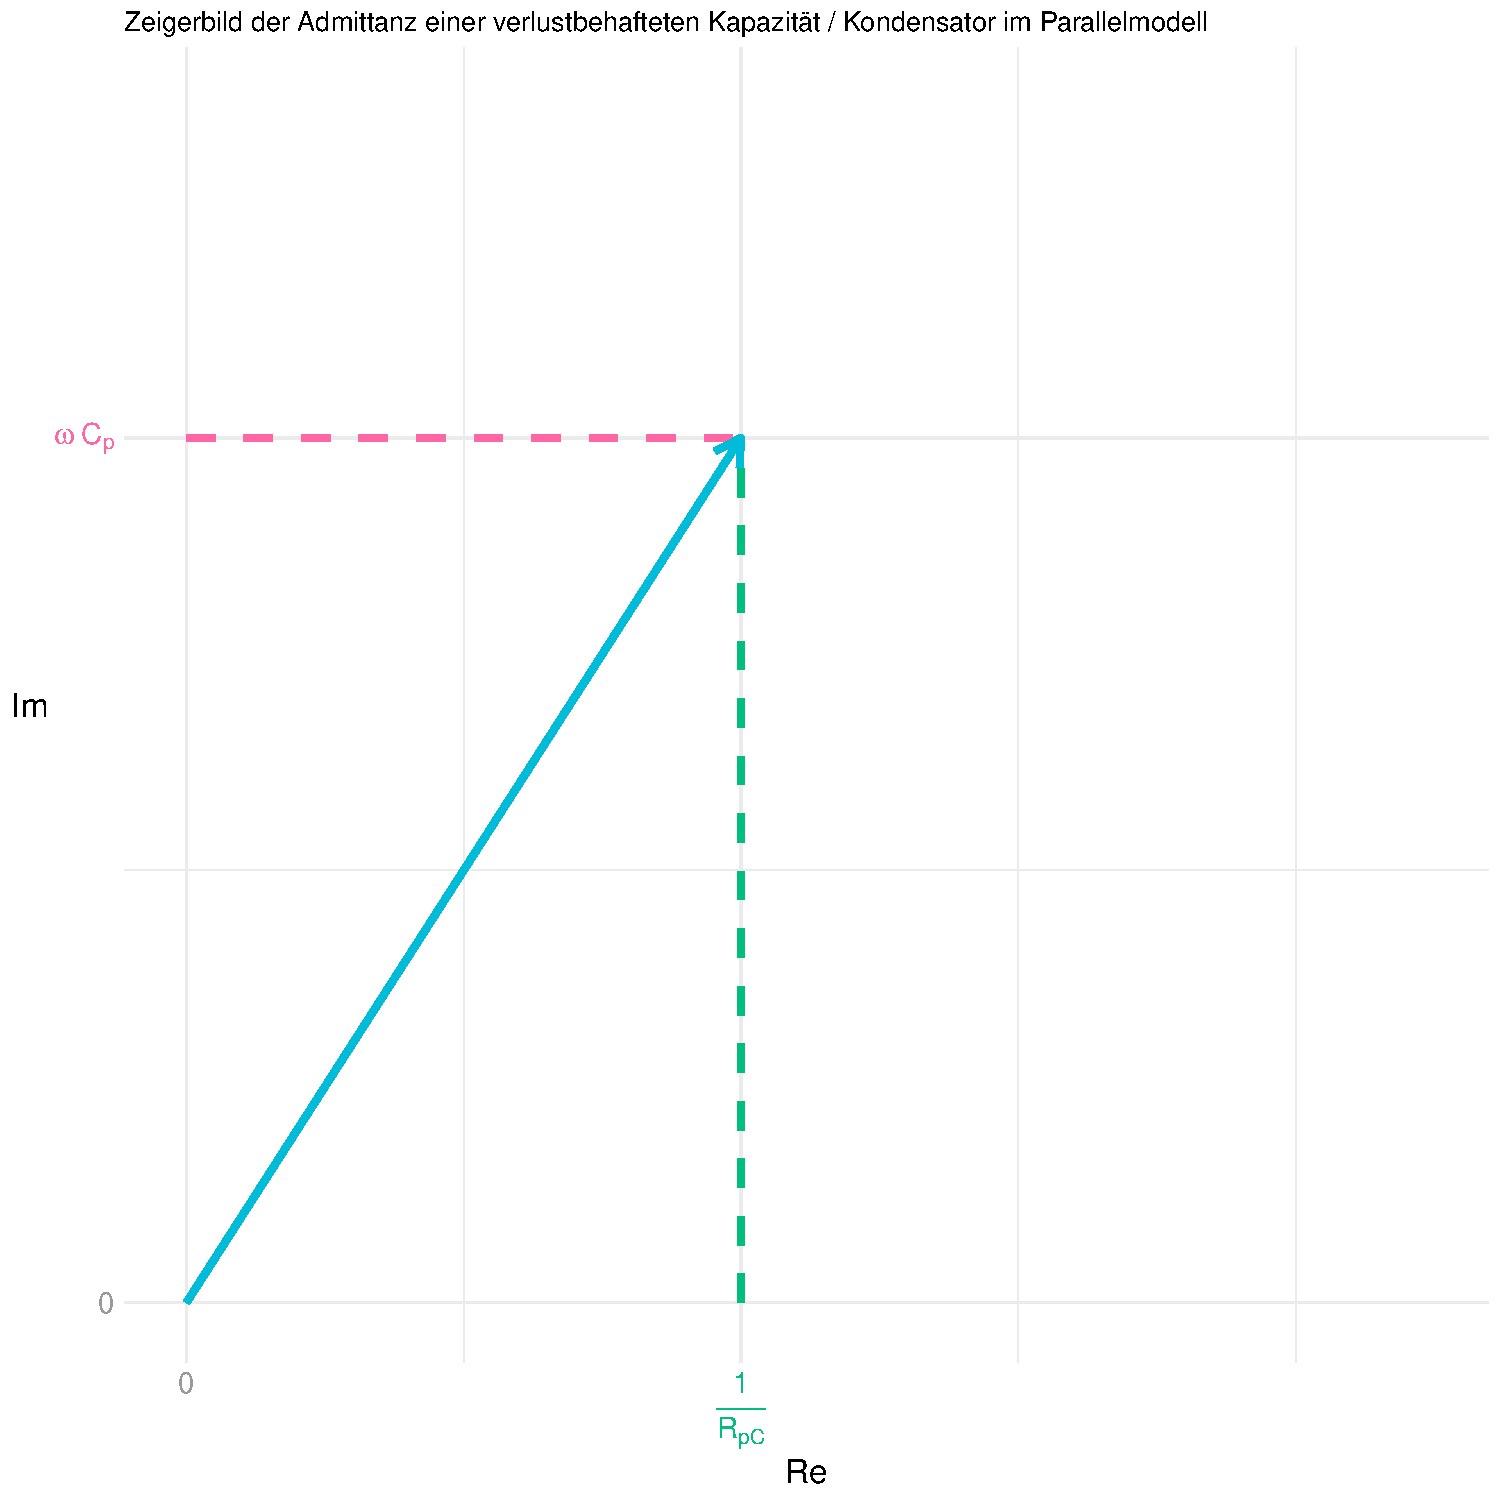
\includegraphics[scale=0.5]{./R/2_5/RC_Zeiger_parallel.pdf}
      \end{center}

      Analog ist der Verlustwinkel  $\delta$ im Parallelmodell der Winkel der Admittanz mit der imaginären Achse:
      $$ d = \tan{\delta} = \frac{ \frac{1}{R_{pC}} }{\omega C_p} = \frac{1}{\omega R_{pC} C_p} $$

      \noindent Demnach ist auch die Güte der Kehrwert des Verlustfaktors:
      $$Q_{Cp} = \frac{1}{d} = \omega R_{pC} C_p $$

      \noindent Für die gleich Frequenz gilt damit:
      $$Q_{C_s} = Q_{C_p} = Q_C$$
      %%%%%%%%%%%%%%%%%%%%%%%%%%%%%%%%%%%%%%%%%%%%%

  %1.6
  \subsection{}
    \begin{center}
      \begin{circuitikz}

        \draw (0,0) to[R, l=$R_{1}$, o-]  (2,0)
                    to[L, l=$L$, -o]      (4,0)
                    to[R, l=$R_2$, *-*]   (4,-2);
        \draw (6,0) to[C, l=$C$, *-*]     (6,-2);
        \draw (0,-2)to[short, o-o]        (8,-2);
        \draw (4,0) to[short, -o]         (8,0);

      \end{circuitikz}

    $$R_1 = 25 \,\ \si{\kilo\ohm}, \,\ R_2=100 \,\ \si{\kilo\ohm}, \,\ C = 1 \,\ \si{\nano\farad}, \,\ L = 0.25 \,\ \si{\henry}, \,\ f = 800 \,\ \si{\hertz}$$
    \end{center}

    \vspace{0.021276873\paperheight}

    \subsubsection*{a)}
      \begin{gather*}
        \underline{Z} = R_1 + j \omega L + \frac{1}{\frac{1}{R_2} + j \omega C} = R_1 + j  \omega L + \frac{\frac{1}{R_2} - j \omega C}{\frac{1}{R_2^2} + \omega^2 C^2}\\
        \underline{Z} = \underbrace{R_1 + \frac{\frac{1}{R_2}}{\frac{1}{R_2^2} + \omega^2 C^2}}_{\text{Realteil (Resistanz)}} + j \underbrace{\left( \omega L - \frac{\omega C}{\frac{1}{R_2^2} + \omega^2 C^2} \right)}_{\text{Imaginärteil (Reaktanz)}}\\
      \end{gather*}

      \begin{gather*}
        \text{Re}(\underline{Z}) = 25 \si{\kilo\ohm} + \frac{1}{100 \si{\kilo\ohm} \left(\frac{1}{(100 \si{\kilo\ohm})^2} + (2 \pi \cdot  800 \si{\hertz} \cdot 1 \si{\nano\farad})^2 \right)} = 104.83 \,\ \si{\kilo\ohm}\\
        \text{Im}(\underline{Z}) = 2 \pi \cdot 800 \si{\hertz} \cdot \left ( 0.25 \si{\henry} - \frac{1 \si{\nano\farad}}{\frac{1}{(100 \si{\kilo\ohm})^2} + (2 \pi \cdot  800 \si{\hertz} \cdot 1 \si{\nano\farad})^2 } \right) = \underbrace{-38.87 \,\ \si{\kilo\ohm}}_{\text{kapazitiv}}
      \end{gather*}

      \begin{gather*}
        \underline{Z} = 104.83 \,\ \si{\kilo\ohm} - j 38.87 \si{\kilo\ohm}
      \end{gather*}

      \subsubsection*{b)}
      %Betrag
      \begin{gather*}
        \mid \underline{Z} \mid
        = \sqrt{ \left(R_1 + \frac{ 1 }{ \frac{1}{R_2} +  \omega^2 C^2 R_2}\right)^2 + \left( \omega L - \frac{\omega C}{\frac{1}{R_2^2} + \omega^2 C^2} \right)^2 }\\\\
        \mid \underline{Z} \mid = 111.8 \,\ \si{\kilo\ohm}
      \end{gather*}

      %\begin{gather*} too large!
        %\mid \underline{Z} \mid
        %= \sqrt{ \left(25 \si{\kilo\ohm} + \frac{ 1 }{ \frac{1}{100 \si{\kilo\ohm}} +  (2 \pi \cdot 800 \si{\hertz} \cdot 1 \si{\nano\farad})^2 \cdot 100 \si{\kilo\ohm}}\right)^2 + \left( 2 \pi \cdot 800 \si{\hertz} \cdot 0.25 \si{\henry} - \frac{2 \pi \cdot 800 \si{\hertz} \cdot C}{\frac{1}{(100 \si{\kilo\ohm})^2} + (2 \pi \cdot 800 \si{\hertz} \cdot 1 \si{\nano\farad})^2} \right)^2 }\\
      %\end{gather*}

      %Phase
      \begin{gather*}
        \phi_{\underline{Z}} = \arctan{\left(   \frac{\omega L - \dfrac{\omega C}{\frac{1}{R_2^2} + \omega^2 C^2}}{R_1 + \dfrac{1}{\frac{1}{R_2} + \omega^2 C^2 R_2} }   \right)} = \arctan{\left(  \frac{-38.87 \si{\kilo\ohm}}{104.83 \si{\kilo\ohm}}  \right)}\\\\
        \phi_{\underline{Z}} = 20.36 \,\ \si{\degree}
      \end{gather*}

  \pagebreak{}
  %1.7
  \subsection{}
    \begin{gather*}
      \intertext{Abgleich bei $U_2 = 0$}
      \frac{R_2}{R_1} = \frac{Z_x}{Z_N} = \frac{\dfrac{1}{\frac{1}{R_x} + j \omega C_x}}{\dfrac{1}{\frac{1}{R_N} + j \omega C_N}} =  \frac{\frac{1}{R_N} + j \omega C_N}{\frac{1}{R_x} + j \omega C_x}\\
      \frac{R_2}{R_x} + j \omega R_2 C_x = \frac{R_1}{R_N} + j \omega C_N\\
      \intertext{Realteilvergleich:}
        \frac{R_2}{R_x} = \frac{R_1}{R_N} \implies R_x = \frac{R_N \cdot R_2}{R_1}
      \intertext{Imaginärteilvergleich:}
        \omega R_2 C_x = \omega R_1 C_N \implies C_x = C_N \cdot \frac{R_1}{R_2}
    \end{gather*}

  %1.8
  \subsection{}
    \begin{gather*}
      \intertext{Abgleich bei $U_2 = 0$}
      \frac{R_2}{Z_N} = \frac{Z_x}{R_3}\\
      \frac{R_2}{\dfrac{1}{\frac{1}{R_N} + j \omega C_N}} = \frac{R_x + j \omega L_x}{R_3}\\
      \frac{R_2}{R_N} + j \omega R_2 C_N = \frac{R_x}{R_3} + j \frac{\omega L_x}{R_3}\\
      \intertext{Realteilvergleich:}
        \frac{R_2}{R_N} = \frac{R_x}{R_3} \implies R_x = \frac{R_2 \cdot R_3}{R_N}
      \intertext{Imaginärteilvergleich:}
        \omega R_2 C_N = \frac{\omega L_x}{R_3} \implies L_x = R_2 R_3 C_N
    \end{gather*}

\section{Versuchsaufgaben}
  %2.1
  \subsection{}
    \begin{center}
      \begin{circuitikz}
        \draw (-2,0) to[R, l=$R_V$,v=$U_{R_{\text{eff}}}$, o-]  (2,0)
                     to[R, l=$R_s$,v=$U_{R_{s_{\text{eff}}}}$]      (4,0)
                     to[L, l=$L$, i=$2 \,\ \si{\milli\ampere}$,v=$U^*_{L_{\text{eff}}}$, -o]   (8,0);
                     \draw (2, -1.618)to[open, v=$U_{\text{L}_{\text{eff}}}$] (8,-1.618);
        \draw (-2, -3)to[open, v=$U_{\text{ges}_{\text{eff}}}$] (8,-3);
    \end{circuitikz}
    \end{center}
    \vspace{0.021276873\paperheight}

    \subsubsection*{a)}
    Bei einem konstanten Strom von $2 \,\ \si{\milli\ampere}$ und einem Vorwiderstand von $1 \,\ \si{\kilo\ohm}$ wurden folgende Werte gemessen:

      \begin{table}[H]
      \begin{center}
      \begin{tabular}{@{}llll@{}}
      \toprule
      $f/\si{\hertz}$   & $U_{R_{\text{eff}}}/\si{\volt}$ & $U_{L_{\text{eff}}}/\si{\volt}$  & $U_{\text{ges}_{\text{eff}}}/\si{\volt}$ \\ \midrule
      20   & 2.003 & 0.1281 & 2.102 \\
      60   & 2.002 & 0.2441 & 2.111 \\
      200  & 2     & 0.7413 & 2.223 \\
      300  & 2     & 1.1063 & 2.369 \\
      500  & 1.998 & 1.838  & 2.785 \\
      1000 & 1.997 & 3.677  & 4.229 \\
      1500 & 1.999 & 5.543  & 5.925 \\ \bottomrule
      \end{tabular}
      \end{center}
      \end{table}

      \begin{center}
        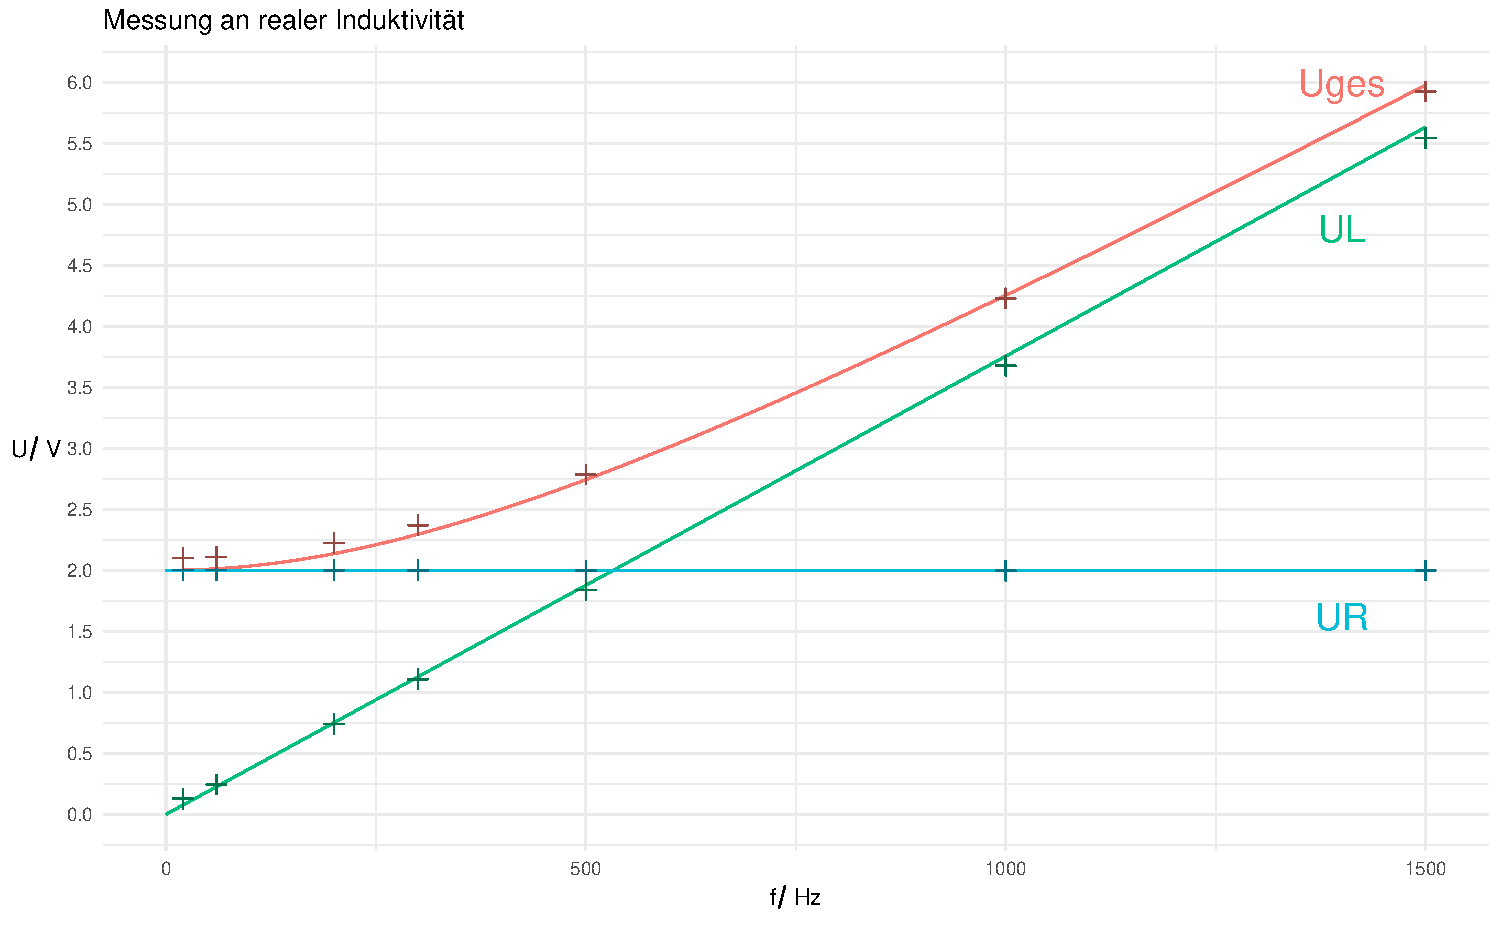
\includegraphics[scale=0.5]{./R/3_1/3_1.pdf}
      \end{center}

     \subsubsection*{b)}
     \noindent Aus diesen wurden dann die folgenden Werte berechnet: (Frequenzen wie oben)
     \begin{gather*}
       \intertext{mit:}
       U_L^* = \sqrt{U^2_L - U_{R_{s}}^2}\\
       U_{R_{s}} = \frac{U_{\text{ges}}^2 - U_R^2 - U_L^2}{2 U_R}\\
       \phi = \arctan{\frac{U_L^*}{U_R}}\\
       \delta = \frac{\pi}{2} - \phi\\
       X_L = 2 \pi f \cdot L\\
       \mid \underline{Z}_L \mid = \sqrt{R_s^2 + X_L^2}
     \end{gather*}
      \begin{table}[H]
      \begin{center}
      \begin{tabular}{@{}lllllll@{}}
      \toprule
      \multicolumn{1}{c}{$U_{R_{s_{\text{eff}}}}/\si{\volt}$}     & \multicolumn{1}{c}{$U_L^*/\si{\volt}$}     & \multicolumn{1}{c}{$R_s/\si{\ohm}$}   & \multicolumn{1}{c}{$\phi/\si{\degree}$}      & \multicolumn{1}{c}{$Q$}       & \multicolumn{1}{c}{$Q_{\text{theoretisch}}$}   & \multicolumn{1}{c}{$L/\si{\henry}$} \\ \midrule
      0.09735 & 0.08326 & 48.67516 & 40.53971 & 0.85528  & 0.77450  & 0.33129   \\
      0.09709 & 0.22396 & 48.54298 & 66.56364 & 2.30685  & 2.32984  & 0.29704   \\
      0.09805 & 0.73479 & 49.02541 & 82.39929 & 7.49394  & 7.68971  & 0.29236   \\
      0.09707 & 1.10203 & 48.53266 & 84.96647 & 11.35352 & 11.65167 & 0.29232   \\
      0.09659 & 1.83546 & 48.29542 & 86.98760 & 19.00243 & 19.51485 & 0.29212   \\
      0.09417 & 3.67579 & 47.08350 & 88.53251 & 39.03484 & 40.03431 & 0.29251   \\
      0.09624 & 5.54216 & 48.12094 & 89.00514 & 57.58579 & 58.75683 & 0.29402   \\ \bottomrule
      \end{tabular}
      \end{center}
      \end{table}

      \begin{table}[H]
      \begin{center}
      \begin{tabular}{@{}lll@{}}
      \toprule
      $\delta/\si{\degree}$  & $X_L/\si{\ohm}$   & $\mid \underline{Z}_L \mid /\si{\ohm}$ \\ \midrule
      49.46029 & 41.63089   & 41.63101         \\
      23.43636 & 111.98117  & 111.98121        \\
      7.60071  & 367.39343  & 367.39344        \\
      5.03353  & 551.01679  & 551.01680        \\
      3.01240  & 917.73011  & 917.73011        \\
      1.46749  & 1837.89700 & 1837.89701       \\
      0.99486  & 2771.08221 & 2771.08221       \\ \bottomrule
      \end{tabular}
      \end{center}
      \end{table}

      \subsubsection*{c)}

      \begin{gather*}
        \underline{Y}_s = \frac{1}{R_s + j \omega L} = \frac{R_s - j \omega L}{R_s^2 + \omega^2 L^2} = \frac{R_s}{R_s^2 + \omega^2 L^2} - j \frac{\omega L}{R_s^2 + \omega^2 L^2}\\
      \end{gather*}

      \begin{gather*}
        \underline{Y}_p = \underbrace{\frac{1}{R_p}}_{\text{Konduktanz}} - j \underbrace{\frac{1}{\omega L_p}}_{\text{Suszeptanz}}\\
        \underline{Y}_s = \underline{Y}_p\\
        \frac{R_s}{R_s^2 + \omega^2 L^2} - j \frac{\omega L}{R_s^2 + \omega^2 L^2} = \frac{1}{R_p} - j \frac{1}{\omega L}\\
        \implies R_p = R_s + \frac{\omega^2 L^2}{R_s^2}\\
        \implies L_p = L \cdot \left( 1 + \frac{1}{Q_s^2} \right)
      \end{gather*}

      \begin{gather*}
        \intertext{Beispiel 1: $f = 20 \,\ \si{\hertz}$}
        R_p = 48.67516 \si{\ohm} + \frac{2 \pi \cdot 20 \si{\hertz} \cdot 0.33129 \si{\henry}}{(48.67516 \si{\ohm})^2} \approx 48.69 \,\ \si{\ohm} \implies \frac{1}{R_p} \approx 0.02054 \,\ \si{\siemens}\\
        X_{L_{p}} = 2 \pi \cdot 20 \si{\hertz} \cdot 0.33129 \si{\henry} \cdot \left( 1+\frac{1}{0.85528^2}\right) \approx 98.543 \,\ \si{\ohm} \implies \frac{1}{\omega L_p} \approx 0.01015 \,\ \si{\siemens}
      \end{gather*}

      \begin{gather*}
        \intertext{Beispiel 2: $f = 1000 \,\ \si{\hertz}$}
        R_p = 47.08350 \si{\ohm} + \frac{2 \pi \cdot 1000 \si{\hertz} \cdot 0.29251 \si{\henry}}{(47.08350 \si{\ohm})^2} \approx 47.91 \,\ \si{\ohm} \implies \frac{1}{R_p} \approx 0.02087 \,\ \si{\siemens}\\
        X_{L_{p}} = 2 \pi \cdot 1000 \si{\hertz} \cdot 0.29251 \si{\henry} \cdot \left( 1+\frac{1}{39.03484^2}\right) \approx 1839.1007 \,\ \si{\ohm} \implies \frac{1}{\omega L_p} \approx 0.0005437  \,\ \si{\siemens}
      \end{gather*}

  %2.2
  \subsection{}
    \subsubsection*{a)}
      Im Versuch wurden die Kapazität $C_N$ und der Widerstand $R_N$ der Maxwellbrücke so eingestellt, dass die Spannung $U_2$ sehr gering wurde. (ca. $4 \,\ \si{\milli\volt}$).\\
      Es wurden die folgenden Messwerte ermittelt:
      \begin{table}[H]
      \begin{center}
        \begin{tabular}{@{}lllllll@{}}
        \toprule
        $f / \si{\hertz}$    & $R /\si{\ohm}$      & $L / \si{\milli\henry}$      & $C_{\text{eingestellt}} / \si{\nano\farad}$       & $R_{\text{eingestellt}}/\si{\ohm}$  & $R2 /\si{\ohm}$   & $R3 /\si{\ohm}$   \\ \midrule
        800  & 54.644 & 292.2 & 292.2 & 18300     & 1000 & 1000 \\
        2000 & 63.29  & 296.7 & 296.7 & 15800     & 1000 & 1000 \\ \bottomrule
        \end{tabular}
      \end{center}
      \end{table}

\end{document}
